\vspace{-0.6em}
\section{Evaluation Pipeline}
\label{sec:evaluation-pipeline}
\vspace{-0.6em}
The previous section describes how expert submissions are collected and converted into verified benchmark instances. This section specifies what happens once a task exists: how it is executed, how the agent interacts with the environment, and how the outcome is scored. The pipeline is organized around an \textbf{uncoupling} of three components (the \emph{task specification}, the \emph{agent}, and the \emph{environment}) so that they can all be easily interchanged.

\noindent \textbf{Terminology.} Throughout the paper we use \emph{task workflow} for an end-to-end professional procedure and \emph{task instance} for one runnable case of a task workflow (one concrete (input, output) pair, sharing the same \texttt{evaluate()} but differing in input and output data). The rare appearance single ``task'' refers to the runnable instance level.

\vspace{-0.6em}
\subsection{Pipeline Architecture}
\label{sec:pipeline-architecture}
\vspace{-0.6em}
\begin{wrapfigure}{r}{0.6\textwidth}
    \vspace{-0.8em}
    \centering
    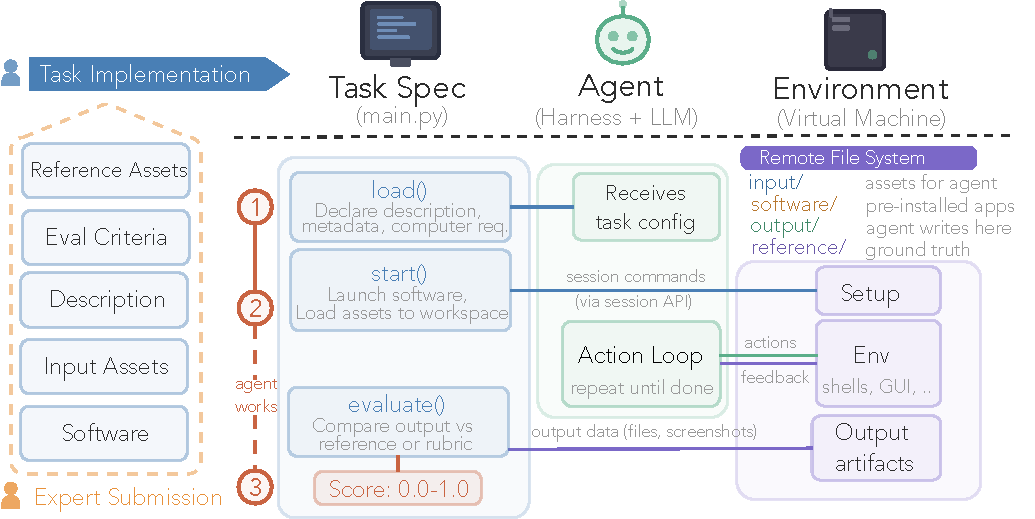
\includegraphics[width=\linewidth]{figures/task-spec.pdf}
    \caption{\textbf{Evaluation pipeline architecture.} Each benchmark instance is defined by a Task Specification (\texttt{main.py}) that orchestrates a three-phase lifecycle (\texttt{load()}, \texttt{start()}, \texttt{evaluate()}) over a remote virtual-machine environment. The agent (harness + model) receives only the task description and metadata, interacts with the environment through an action loop, and produces output artifacts that the specification scores against references or rubrics.}
    \label{fig:task-spec}
    \vspace{-0.8em}
\end{wrapfigure}

Figure~\ref{fig:task-spec} illustrates the end-to-end evaluation pipeline. A benchmark instance is realized through three decoupled components that interact via well-defined interfaces. The \textit{task specification} is an executable \texttt{main.py} encoding the five elements supplied during construction (description, input assets, target software, reference assets, evaluation criteria) and exposing three lifecycle functions: \texttt{load()} declares the task and compute requirements, \texttt{start()} provisions the VM into a deterministic starting state, and \texttt{evaluate()} scores the agent's output in $[0, 1]$. The \textit{agent} (a harness orchestrating a foundation model) receives only the task description and metadata, then runs an action loop over screenshots, shell output, mouse and keyboard, file edits, and API calls until it terminates. The \textit{environment} is a remote virtual machine with a canonical four-directory layout: \texttt{input/} (read-only assets), \texttt{software/} (pre-installed applications), \texttt{output/} (the agent's sole writable target), and \texttt{reference/} (ground-truth artifacts hidden from the agent and used only for scoring). This decoupling lets any agent that conforms to the action interface be evaluated on any task, and a single specification be deployed across cloud VMs or local containers without modification. Per-component interfaces and the directory contract are detailed in Appendix~\ref{app:pipeline-architecture}, with the lifecycle protocol in Appendix~\ref{app:task-spec-protocol}.

\vspace{-0.4em}
\subsection{Agent Architecture: From CLI/GUI-agents to Generalist CUA}
\label{sec:agent-architecture}
\vspace{-0.4em}
The tasks in ALE require agents that can read GUI screens, type in dialog boxes, execute shell commands, write and debug code, invoke APIs, and manage long-running sessions, often within a single task workflow. No single existing agent family covers this surface natively, so the benchmark targets a broader agent class that we make explicit here, together with how the prevailing harness architecture is extended to reach it.

\begin{figure}[t]
    \centering
    \begin{minipage}[b]{0.42\textwidth}
        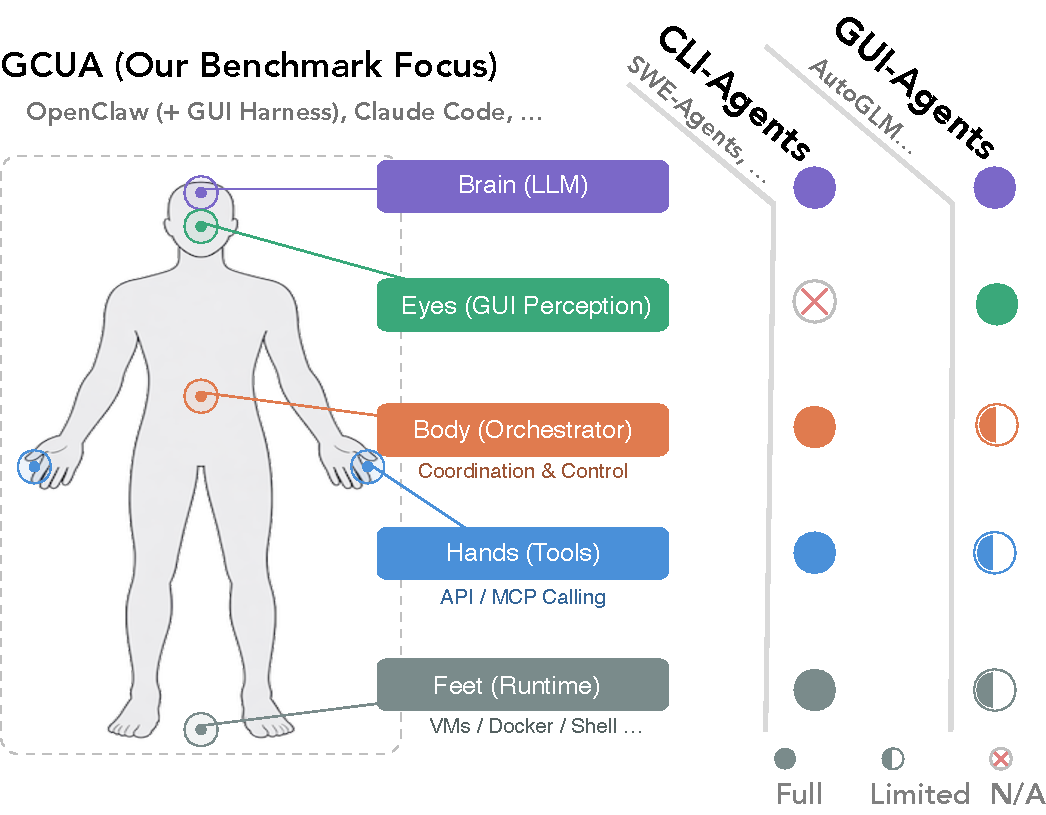
\includegraphics[width=\textwidth]{figures/agent-body.pdf}
        \caption{\textbf{Agent capability taxonomy.} Five functional layers define an agent's operational surface. Generalist CUA-agents (GCUA) possess full capability across all layers; CLI-agents lack visual perception (Eyes); GUI-agents have limited orchestration, tool use, and runtime access (Body, Hands, Feet).}
        \label{fig:agent-body}
    \end{minipage}
    \hfill
    \begin{minipage}[b]{0.55\textwidth}
        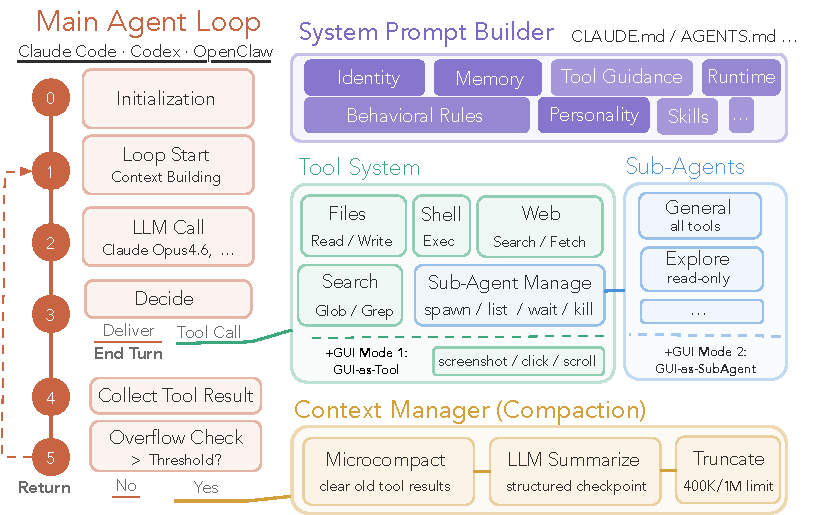
\includegraphics[width=\textwidth]{figures/agent-harness.pdf}
        \caption{\textbf{Typical GCUA harness architecture.} The main agent loop (left) cycles through context building, LLM inference, action decision, tool execution, and overflow management. The system prompt builder, tool system (including GUI harness via MCP), sub-agents, and context compaction manager are shared across mainstream harness implementations.}
        \label{fig:agent-harness}
    \end{minipage}
    \vspace{-1.2em}
\end{figure}

We decompose an agent's operational capabilities into five functional layers (Figure~\ref{fig:agent-body}): \textbf{Brain} (LLM reasoning and planning), \textbf{Eyes} (GUI perception via screenshots), \textbf{Body} (orchestration and control flow), \textbf{Hands} (structured tool invocation), and \textbf{Feet} (the runtime substrate on which actions take effect). This decomposition exposes a clean split among existing families. Traditional \textbf{CLI-agents} such as SWE-agent~\citep{yang2024swe} and ForgeCode~\citep{tailcall2024forgecode} have full Brain, Body, Hands, and Feet but lack Eyes by construction; framework-style agents such as OpenClaw are not strictly CLI-only, yet they ship without a native GUI module. \textbf{GUI-agents} built on vision-language action models cover Brain and Eyes but expose only shallow Body, narrow Hands (mostly mouse and keyboard), and restricted Feet, leaving them unable to write code, manage files, or sustain long workflows. ALE's task workflows demand the union of both surfaces, so the agent class the benchmark evaluates is the \textbf{Generalist CUA-agent} (GCUA): an agent with full capability across all five layers. \textbf{We adopt the ``Generalist'' qualifier deliberately, because the industry often equates CUA-agents with GUI-agents; this conflation is incomplete.} 

The harness layer that mediates model and environment has converged toward a structure rich enough to support GCUA. Early agents revolved around a thin reasoning loop in the style of ReAct~\citep{yao2023react} (interleaved \textit{Think} and \textit{Action} steps); contemporary harnesses such as Claude Code~\citep{anthropic2025claudecode}, Codex~\citep{openai2025codex}, and OpenClaw share a richer macro-architecture that we treat as representative of the modern agent-harness layer (Figure~\ref{fig:agent-harness}): a main agent loop, a modular system prompt builder, a unified tool system, sub-agent dispatch, and a context compaction manager for long-horizon runs. Because these harnesses are CLI-native, lifting them to GCUA reduces to adding GUI capability. We use two modes: \textbf{GUI-as-Tool} exposes GUI operations as ordinary tools in the main loop, while \textbf{GUI-as-SubAgent} delegates GUI interaction to a specialized vision-language sub-agent. We currently reserve GUI-as-SubAgent for models without native vision input, such as DeepSeek V4~\citep{deepseek2026v4pro}. Our primary benchmark evaluation uses GUI-as-Tool to measure integrated visual reasoning and action over the full task. Component-level harness internals are deferred to Appendix~\ref{app:agent-harness}.

\vspace{-0.6em}
\subsection{Evaluation Modes}
\label{sec:evaluation-modes}
\vspace{-0.4em}
The deliverables that \texttt{evaluate()} must score are highly heterogeneous (CAM toolpaths, financial workbooks, 3D meshes, game world states, rendered screenshots, structured filings, free-text reports). Rather than impose a single scoring metric, ALE composes every task's evaluation along two orthogonal axes. \textbf{(i) Comparison form}: task authors pick from a small palette of artifact modes: exact / hashed values, structured numeric or tabular fields with manifest-driven tolerances, geometric surface or point-cloud distances, visual appearance (vision-LLM judge), behavioral world state under a fixed input trajectory, and free-text rubric scoring. \textbf{(ii) Composition}: the per-artifact signals are combined either by a \emph{gate-and-score} pattern or by averaging a binary checklist or per-file scores. Gate-and-score is the most common pattern: a binary precondition (e.g., ``no toolpath collision,'' ``file parses without error'') must pass before a continuous quality metric (surface deviation, dimensional accuracy, etc.) is evaluated; failure on the gate forces the task score to $0$ regardless of partial progress on other criteria. The full mode taxonomy with per-task-workflow assignments, helper APIs, and worked examples are given in Appendix~\ref{app:evaluation-modes}.

ALE \textbf{deliberately avoids LLM-as-judge} wherever a deterministic alternative exists; a task workflow whose only proposed scoring path is ``ask a model whether the result looks correct'' is rejected at QC and re-engineered to expose a checkable artifact. The minority of task workflows that genuinely require an LLM judge (video clip, game screenshot, rendered scene, etc) are scored not by general-purpose holistic prompts but by narrow, evidence-anchored yes/no probes whose answers code aggregates into the score. Each task workflow exposes a list of task instances (e.g., the 18 workpiece instances in \texttt{manufacturing/gcode}) that share a single \texttt{evaluate()} but differ in input and reference.
